
\chapter{Introduction}

\section{Entry Level Requirements}
In this module we assume that you are familiar with:
\begin{itemize}
\item \emph{Linear Algebra.} You should be familiar with matrix vector manipulations.
  You should know what eigenvalues and eigenvectors are.
\item \emph{Basics of Statistics.} You should be aware of the concepts of probability,
  expectation, variance and the Gaussian distribution. Most of these concepts will
  be reviewed briefly.
\item \emph{Python Programming.} You should be familiar with Python data structures,
  functions and classes. You should know what numpy arrays are and be able to slice
  them.
\end{itemize}  

\section{Warning}
The material presented here is intended to provide the theoretical framework
for the later material. It is not suitable for the analysis of real world data without
further reading. We have not discussed the need for more robust inference
when data contains \emph{outliers}. At the very least, you should consult
section 7.4 of \cite{murphy2012}. In Unit 4 you may find useful techniques
to model outliers as a mixture of different processes.

  
\section{Learning Outcomes for Unit 1}
In this unit we will revise some of the basic notions of statistics. In particular
you should be  familiar with:

\begin{itemize}
\item Fundamental concepts of statistics: stochastic variables,
  probability distributions, probability densities.

\item Joint and marginal distributions, Bayes' rule.
\item Likelihood.
\item Maximum likelihood estimation.
\end{itemize}

We will then go on to study a Bayesian interpretation of coin throws. You
should be able to:

\begin{itemize}
\item Use the Bernoulli process as a model for coin or dice experiments.
\item Explain the relationship between the binomial and the Bernoulli distribution.
\item Give a Bayesian interpretation of a Bernoulli process using the Beta distribution.
\end{itemize}

\chapter{Revision of Probability Concepts}
\section{Basic Concepts}
\subsection{Probability}

Obligatory examples of stochastic processes are coin flipping and dice throwing.
A coin lands on head or tails, these are the possible \emph{outcomes}. The set of all
outcomes is the \emph{state space}.  The state space formed by the outcome of a dice
throw is $\left\{ '1', '2', '3', '4', '5','6' \right\}$, where $'1'$ stands for:
'the dice landed such that the side which has one marker is on top'. $'1'$ is shorter.
Sometimes, the numerical value is relevant, e.g. in many board games, and the
state space is considered to be the numbers $\{1,  2, 3, 4, 5, 6\}$ when there is no
risk of confusing the numerical value with its actual realisation. The state space
of the outcome of throwing two dice will be $\{1, \cdots, 36 \}$, etc.
State spaces can be \emph{discrete} or \emph{continuous}: the time of arrival for the
next train at a platform can take any value between 1 ns to two years, at least in the UK.

  
\emph{Stochastic variables} are variables representing potential outcomes of a
probabilistic event, an event to which we attribute a certain amount of
\emph{uncertainty}. The process of realising this event is called a \emph{stochastic process}.
Upon the realisation of the event, the stochastic variable associated
with the event has assumed as a value one of the possible elements of the
state space associated with the stochastic process at the exclusion of all other
possible elements. Stochastic variables are denoted by capital letters. In the context
of a coin flip, the statement $P(X='T') = 0.5$ usually means that the outcome
of the next coin flip results in 'tails' is 50 \%. Here $X$ is shorthand for
'the outcome of a coin flip'. The context where a stochastic variable
acquires its meaning must be specified very carefully. The outcome of a coin throw
is called an \emph{event}. Events are indicated by capital letters. So $A$ can stand
for: '6 came up when the dice was thrown', which is an  event. The value of the
outcome is a \emph{realisation}, so in the previous example '6' is the realisation
of the stochastic process of dice throwing for that particular event. A set of
outcomes is called a \emph{sample}, the set size is called
the \emph{sample size}.

A \emph{probability distribution} is a set of probabilities defined over a state
space such that each element of state space has one probability associated with it.
The sum of all probabilities must add to one.  
For a discrete distribution we can label the state space with an index $i$, and
define the probability $p_i$ associated with outcome $i$. We have:
\begin{enumerate}
\item $0 \le p_i \le 1$
\item $\sum_i p_i = 1$ 
\end{enumerate}


  
If we generate or collect new events that are distributed according to some
probability distribution, we are said to \emph{to sample} the distribution.
  
The amount of uncertainty by which a particular outcome is realised is quantified
by a numerical value, a \emph{probability}. The probability of a particular outcome
is a real number in the interval $[0,1]$, where $0$ represents absolute certainty
that the outcome will not be realised and $1$ represents absolute certainty of its
realisation. The intrinsic meaning of such probabilities is subject of an ongoing
debate.
  
  
The \emph{frequentist} interpretation considers probability as the
ratio of two numbers observed in a large number of repeated experiments. For
example for a particular dice, one can throw a large number of times, say $N$ times.
The probability of the even '1' is approximately given by the number of times
that '1' came up, divided by $N$. The frequentist imagines that this experiment
in principle could be performed an arbitrary large number of times and that the
observation of the ratio of outcomes would converge to a real number that would
then constitute \emph{the} probability. Although intuitively appealing, there are
problems with this definition. A real dice might wear in the process of throwing,
thereby slowly changing the propensity for '1' to come up, thereby creating tension
between the mathematical process of taking the limit and the real world implementation
of it. It also assumes that the experiment can be prepared identically without
physical attrition of the dice. But a human thrower would tire, potentially subtly
altering the probability of realising '1'. Maybe the human does not want to throw '1'
and is somehow capable of influencing the odds slightly. Mechanical processes for
throwing dice would suffer from wear and tear again. It turns out to be surprisingly
hard to create a rigorous definition of the concept of probability. The frequentist
approach dominates in high school teaching, possibly indicating that despite the
difficulty in establishing a rigorous footing, the concept has intuitive appeal.

The \emph{Bayesian} interpretation considers probability a quantitative measure of
subjective believe. If I believe a coin is fair - and this believe is subjective,
because I may distrust the person who provided me with it -,
then the probability for an outcome '1' is $\frac{1}{6}$. In the Bayesian
view this \emph{prior} belief can be modified in the face of experimental outcomes
in a very specific way that we will discuss in detail in Sec. \ref{sec-bayes}.
Advocates of the Bayesian approach argue that some situations where we routinely
assign probabilities to potential outcomes are not repeatable on principle. If I
already have taken an exam, but am uncertain about its outcome, I may assign a
probability that I passed it, say 30 \%. This indicates a degree of pessimism, but
the outcome is determined and the situation is clearly non repeatable because I now
know the questions for this particular exam. I would probably do better on it next
time, or if I were not allowed to prepare for it in the interest of frequentist purity
I might have forgotten the subject matter. Probability here, a Bayesian would argue,
is more the quantification of a subjectively held belief, rather than a number
to determined by repeating the exam a large number of times, something that is
not possible, even in principle. Moreover, the outcome is already determined. It is
just that I don't know the outcome. Does it make sense to assign a number at all?
Clearly, if I start to compare notes with other students I may realise that I actually
performed better than I believed initially and my probability of 30 \% is unreasonably
low. So apparently, in the face of new information I can lower or raise this
probability. Jaynes \cite{jaynes2003probability} gives a fascinating discussion of the Bayesian
view point which argues that not only probabilities can be considered to be
quantitative measures of subjective believe, but that by assumption of a number
of reasonable, intuitively obvious rules for combining these believes one can
arrive at the sum and product rule to be discussed below \footnote{The first three chapters of Jaynes' book are
available online at \url{https://bayes.wustl.edu/etj/prob/book.pdf}}. We will rely on these rules
extensively and frequentists and Bayesians do not disagree on them so we will not
pursue the Bayesian interpretation of these rules. However, anyone who wants to make
a career in machine learning is recommended to get acquainted with these ideas at some
point.


  
\subsection{Expected Value and Variance for Discrete Variables}

If a function f(x) is defined over a discrete states space, i.e. for each $x_i$ in the state space
we know $f(x_i)$, then the \emph{expectation value} is:

\begin{equation}
\mathbb{E}[f] = \sum_i p(x_i)f(x_i).
\end{equation}

The \emph{variance} is :

\begin{equation}
\mbox{var}[f] = \mathbb{E}[(f(x) - \mathbb{E}[f(x)])^2],
\end{equation}

which can also be written as:

$$
\mbox{var}[f] = \mathbb{E}[f(x)^2] - \mathbb{E}^2[f(x)]
$$

(you should be able to prove this).

The expected value indicates the centre of gravity of the probability distribution, the variance is
a measure for how spread out the probability is. In general, the larger the variance, the less representative
the expected value is for a typical event.

The $n$-th \emph{moment} of a discrete distribution is given by:

$$
\mu_n = \sum_i p(x_i) f(x_i)^n,
$$

so

$$
\mathbb{E}[f] = \mu_1
$$

and

$$
\mbox{var}[f] = \mu_2 - \mu^2_1
$$

Higher moments give information about whether a distribution is skewed, and in general
the more moments are known, the more accurate a distribution can be characterised. Some distributions,
as we will see are only characterised by a few moments.

\subsection{Examples of Discrete Distributions}

We have already seen examples of distributions of discrete variables: dice throwing and coin tossing. The Bernoulli process can be considered as a model
of throwing a coin. Its state space is the two-element set $\{0, 1 \}$. The process is defined by:

\begin{equation}
\mbox{Ber}(x \mid \mu) = \mu^x(1-\mu)^{1-x},
\end{equation}

for $0 \le \mu \le 1$.
  
In one neat formula this expresses the fact that the probability for obtaining $x=1$ is given by $\mu$, and that the probability for $x=0$ is given by $1 - \mu$. This
process can be used to model  a fair coin for $\mu = 0.5$ and one with bias for other values.
You should be able to establish that:

\begin{align}
\mathbb{E}[x] & = \mu \\
\mbox{var}[x] & = \mu(1 - \mu) \nonumber
\end{align}

Another important distribution, closely related to the Bernoulli process, is the binomial distribution. It can emerge, for example, in the context of a random walk. Assume
that we start at position 0 and can move one step to the right with probability $\mu$ or stay in place with probability $1 - \mu$. Each individual step can be modelled by a Bernoulli process. A natural question to ask is where do we end after $N$ steps. It is clear that the position must be somewhere between $-N$ and $N$, assuming that each step increments (decrements) our position coordinate by 1. What would the distribution look like? This position is modeled by a binomial process:

\begin{equation}
\mbox{Bin}(m,N \mid \mu) = \left( \begin{array}{c} N \\ m \end{array} \right) \mu^m(1- \mu)^{N-m}, 
\end{equation}

where

\begin{equation}
\left( \begin{array}{c} N \\ m \end{array} \right) = \frac{N!}{(N-m)!m!}
\end{equation}

In order to end up at position $m$ we need $m$ moves to the right. Since we assume that moves are independent the probability of any
sequence containing $m$ moves to the right and $N-m$ non moves
is simply $\mu^m(1-\mu)^{N-m}$. There are $\left( \begin{array}{c} N \\ m \end{array} \right)$
such moves as this is the number of ways that we can select $m$ objects out of a set of $N$ total objects (with replacement).


\begin{figure}[!ht]
\begin{center}
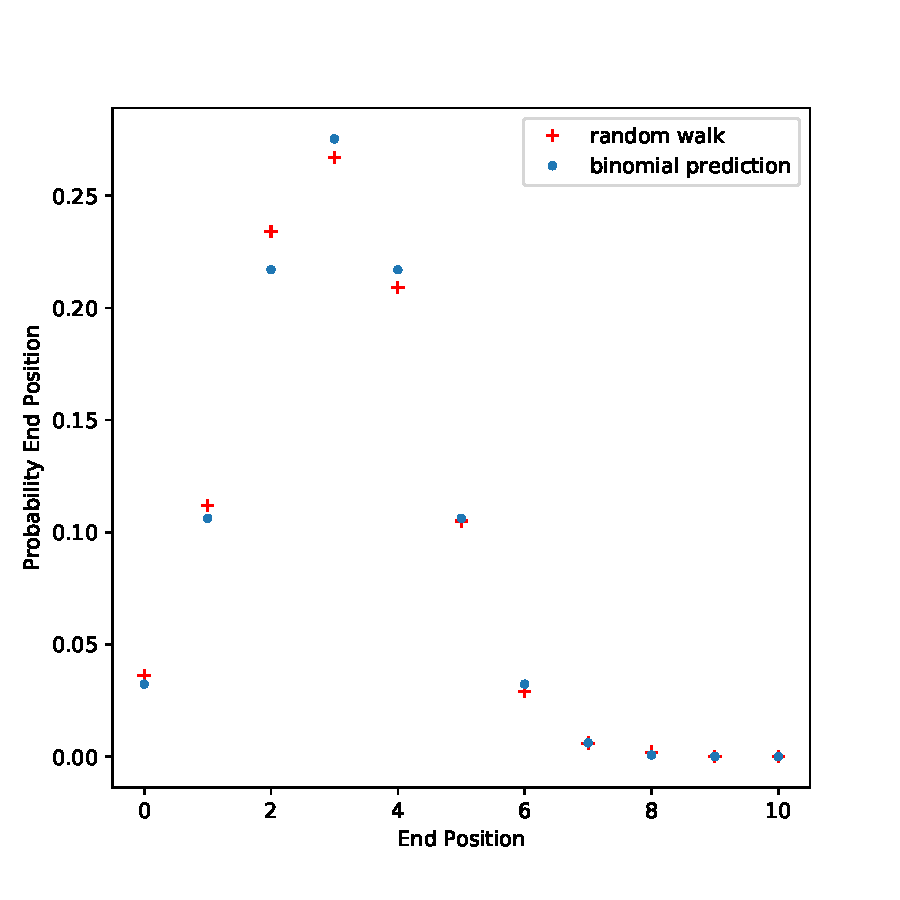
\includegraphics[width=0.7\textwidth]{rw.pdf}
\end{center}
\label{fig-rw}
\caption{Example of a random walk as a binomial process. In total 10 steps are considered. For each step, there is a probability $\mu$ to move to the right and a probability 1 - $\mu$ to stay in place. This 10 step process is simulated with a Bernoulli process and the end position is recorded 1000 times. A histogram of the end positions is normalised so as to produce an observed probability density function ('random walk'). The probability density can also be calculated as a binomial process $\mbox{Bin}(10,0.3)$. This distribution is also shown ('binomial prediction').}
%\alt{Example of a random walk as a binomial process.}
 \end{figure}

Loosely speaking, the binomial distribution emerges if we are interested in the distribution of the sum of a fixed number of outcomes of Bernoulli distribution events.
Other examples are the sum of the outcome of two dice throws, which is essential in many board games.


\section{Continuous Probability Distributions}

The outcome of some stochastic processes can be in a continuous state space. The probability of a patient dying in the next 5 years is not  restricted to
discrete values, and a probabilistic statement about the adult height a child is likely to grow to obviously requires a continuous interval, something like
$[0.5, 2.3]$. Probability density functions can be defined on complex sample spaces. For simplicity, here we will just consider a single connected interval in one dimension,
which may be infinite, closed, open or half open. More complex situations will be discussed when needed.
On this interval we will consider a \emph{probability density function}. These functions are not necessarily smooth or even continuous. Their most important properties
are:

\begin{enumerate}
\item $\int^b_a f(x) d x = 1$ for interval $I$, where $I = (a,b), [a, b), (a, b], or [a,b]$.
\item For every sub interval of $I$, $I_0$, $0 \le \int_{I_0} f(x)dx \le 1$.
\item Summed over all sub intervals, the probability must add to 1. We will remain deliberately vague about the term 'all sub intervals'. It can be well defined,
      but is highly technical.
\end{enumerate}

The second condition implies that for all $x \in I, f(x) \ge 0$. It does \emph{not} imply $f(x) < 1$. A probability density  can attain arbitrarily large values,
as long as its integral on any subinterval of $I$ is less or equal to one.

\subsection{Expectation and Variance of a Continuous Distribution}

For a continuous probability distribution $p(x)$ defined on interval $I = [a,b]$, the expectation of an arbitrary function is:

\begin{equation}
\mathbb{E}[f(x)] = \int^b_a f(x)p(x) dx
\end{equation}

The variance is defined as:

\begin{equation}
  \mbox{var}[f(x)] =  \mathbb{E}[(f(x) - \mathbb{E}[f(x)])^2].
\end{equation}


If the probability density function has a single peak, the value for which it occurs is the \emph{mode} of the distribution. A population density function
with a single peak is called \emph{unimodal}. If more than one maximum occurs, the function is called \emph{multimodal}.
  
The expectation value gives an indication where the bulk of the probability mass is residing. The variance gives an indication as to how widely the probability
mass is distributed. For a distribution function with a single narrow peak, the variance will be small, for a broader peak, which must be flatter as the
total area under the curve must be equal to 1, the variance will be larger. also multimodal distributions tend to have larger variance than unimodal once for peaks of
comparable width.

The expectation value and variance are simple expressions in the \emph{moments} of the distribution function. The $n$-th moment, $m_n$ is defined
as:

$$
m_n = \int (f(x))^np(x) dx
$$
  
\subsection{Example: Uniform distribution}

\begin{figure}[!h]
\begin{center}
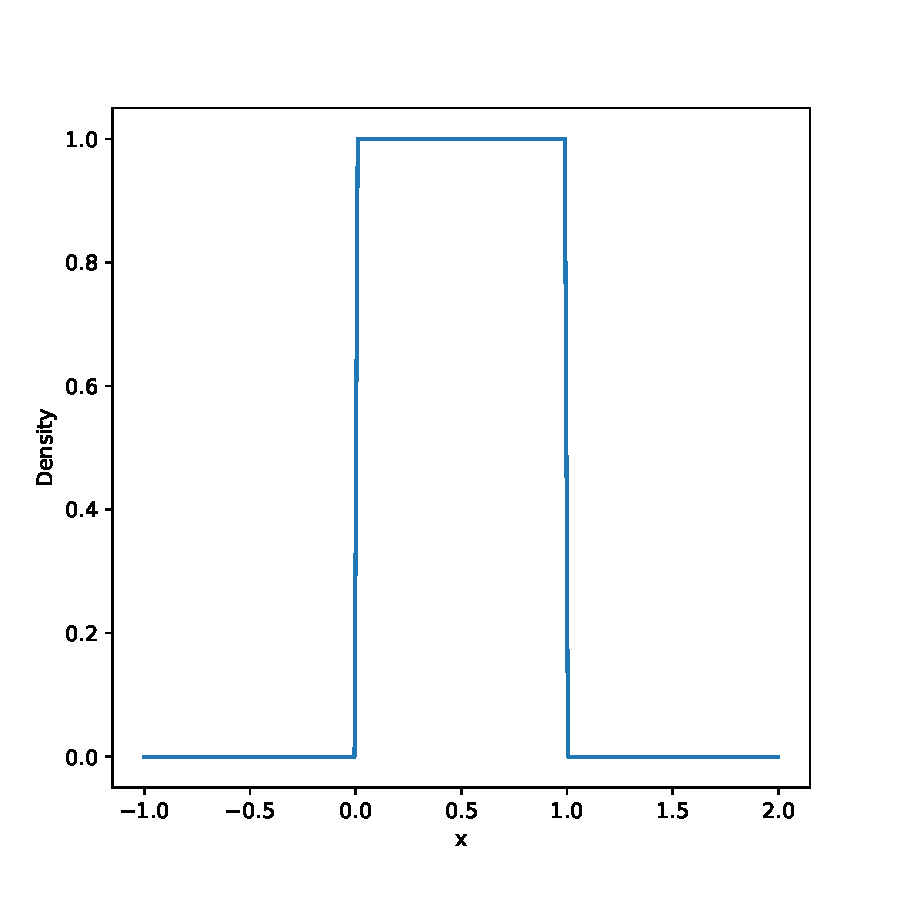
\includegraphics[width=0.7\textwidth]{uniform.pdf} 
\end{center}
\caption{Top: the uniform distribution.}
\label{fig-uniform}
\end{figure}

The function $f(x) = 1$ on $[0,1]$ (Fig. \ref{fig-uniform} is a probability density function, expression the fact every number is equally likely to be sampled
(technically with probability 0). It easy to check that is satisfies the two requirements given above. Some care has to be taken in interpreting probabilities compared
to discrete probabilities. It makes sense to specify an interval and ask what the probability is that the next sample value will be in that interval. E.g. the
probability to sample a number from the uniform distribution in the interval $[0.1, 0.2]$ is equal to 0.1. The probability to sample the number $\pi$ exactly is 0.

It is not possible to write computer algorithms that generate truly random numbers, but a number of pseudo algorithms is known that generate sequences of numbers that
\emph{appear} random enough to evade tests that try to establish whether there is structure in the data that was generated. These algorithms simulate the uniform
distribution, so it plays a central role in simulation random processes. In the activity \emph{Simulating Stochastic Processes}, you will experiment with how you can simulate arbitrary distributions
based on \emph{random number generators} that sample the uniform distribution.

\subsection{Example: Gaussian or Normal Distribution}

\begin{figure}[!h]
\begin{center}
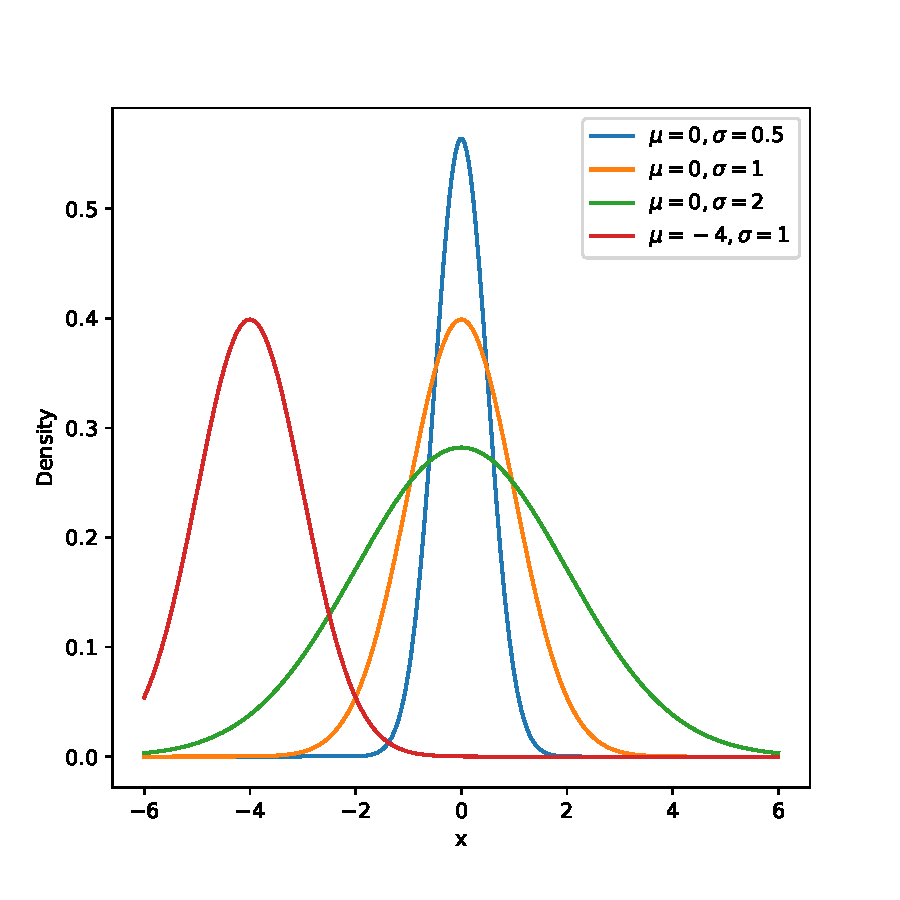
\includegraphics[width=0.7\textwidth]{gauss.pdf} 
\end{center}
\caption{The Gaussian or normal distribution for several values of \( \mu \) and \( \sigma \).}
\label{fig-gauss}
\end{figure}

Examples of the Gaussian distribution are shown in Fig \ref{fig-gauss}. A closed formula exists:

\begin{equation}
  \mathcal{N}(x \mid \mu, \sigma^2)  = \frac{1}{\sqrt{2\pi \sigma^2}}e^{-\frac{1}{2\sigma^2}(x-\mu)^2}
\end{equation}

The distribution has a bell shape, which is wider or narrower dependent on parameter $\sigma$, the variance. Its mode (peak) is at $x = \mu$, the function is symmetric around
this value. One can show that:

\begin{align}
\mathbb{E}[\mathcal{N}(x \mid \mu, \sigma^2)] & = \mu \\
\mbox{var} [\mathcal{N}(x \mid \mu, \sigma^2)] & = \sigma^2 \nonumber 
\end{align}


\subsection{Likelihood}

Many models of stochastic processes are \emph{parameterised}.
We have already seen several examples of parameterised distributions. For example, the Bernoulli process, which
is governed by a parameter $\mu$.
    

When $P(X \mid \mu)$ is considered to be a function of $X$ we refer to it as a probability distribution. Probabilities sum to one:

$$
\sum_i P(X = x_i \mid \mu) = 1,
$$

where in this particular example $x_0 = '0'$ and $x_1 ='1'$. Probability distributions are \emph{normalised}.


We will see that it is sometimes useful to consider this object to be a function of $\mu$. It is then called a \emph{likelihood}. An
importance difference between probability and likelihood  is that normalising the distribution with respect to the likelihood parameter usually does not make sense.
In general, we would consider $\mu$ a continuous variable: $\mu \in [0, 1]$. There is no sensible way to define the normalisation of a likelihood and no
need to do so.
  
An interesting question is now: 'Given a number of observed coin tosses, can I \emph{infer} the parameter $\mu$?' A direct question might be: 'is this coin fair'? If
we can infer that the $\mu = 0.5$, the answer would be yes. Someone inclined  to gamble and intent on maximising the profit might even go further and ask:
'can I predict future series of coin throws and thereby place my bets optimally?'. Such a person would be intent on \emph{prediction} and might not even care
about the particular value of $\mu$ or the question whether the coin is fair, but only about predictions that are as accurate as possible.

  
The question of how to infer parameters from data is central in machine learning and will be discussed throughout the module.

\subsection{Maximum Likelihood Estimation}

Maximum Likelihood Estimation (MLE) is the most widely used method to infer the parameters of a distribution when given a certain dataset. We will illustrate the technique
with a number of examples.

\noindent{\bf Example: Bernoulli Process.}

Imagine that we have observed a sequence of 0s and 1s, e.g. 000101010001, which we call the data set $\mathcal{D}$.

\begin{itemize}
\item We assume that these events have been independently generated by the same Bernoulli process (independently identically distributed; \emph{iid}).
\end{itemize}

The probability for creating this particular sequence can be expressed in the unknown parameter, since the probability for each event is known and the events are independent.
We find:

$$
P(\mathcal{D} \mid \mu ) = (1-\mu)^3\mu(1-\mu)\mu(1-\mu)\mu(1-\mu)^3\mu = (1 - \mu)^8 \mu^4
$$

In MLE we consider the left hand side as a function of $\mu$, i.e. as a likelihood and will look for the value of $\mu$ that maximises the likelihood associated with the
observed data. To solve this problem, we first note that the general case of a sequence of $N$ data points with $N_1$ observations is hardly more complicated:

\begin{equation}
P(\mathcal{D} \mid \mu ) = \mu^{N_1}(1 - \mu)^{N - N_1}
\end{equation}

We want to maximise this quantity. In order to do this we will take the logarithm, using the monotony
of the logarithm: the value for $\mu$ that maximises the likelihood also maximises the log likelihood, which is a simpler expression.

$$
\ln P(\mathcal{D} \mid \mu) = N_1 \ln \mu + (N - N_1) \ln (1 - \mu)
$$

We find the value of $\mu$ that maximises the likelihood, $\mu_{ML}$ by:

$$
\frac{d \ln P(\mathcal{D} \mid \mu) }{d \mu} \mid_{\mu = \mu_{ML}} = 0
$$

this works out as:

$$
\frac{N_1}{\mu_{ML}} - \frac{N - N_1}{1 - \mu_{ML}} = 0,
$$

solving for  $\mu$:

\begin{equation}
\mu_{ML} = \frac{N_1}{N}
\end{equation}
  

The second derivative is:

$$
-\frac{N_1}{\mu^2} - \frac{(N - N_1)}{(1 - \mu)^2}
$$

Since $N - N_1 > 0$ and $N >0$, this term is negative. Therefore $\mu = \frac{N_1}{N}$ is a maximum of the log likelihood, moreover it is the only mnaximum. We conclude that this value of $\mu$ maximises the likelihood.

Intuitively, this estimate for $\mu$ makes sense. When the estimate is made on a large amount of data, it will approach the true value of $\mu$, but the MLE approach is a point
estimate for $\mu$ without any quantification of uncertainty. This is a substantial drawback when inference is done on small datasets. We will address this issue when we
confront the MLE approach with Bayesian inference in Sec. \ref{sec-bayesexample}.


\chapter{Multivariate Distributions and Bayes' Theorem}

` \subsection{Joint Probabilities}
  If we throw not one but two dice, the size of our state space increases from 6 to 36,
  as there are 36 different combinations which the pair of dice can realise. Note that
  here a distinction is being maintained between the combined events where '1' is the
  result of the first die and '2' the result of the second die, as opposed to
  a '2' for the first die and a '1' for the second die.

  %Often we are interested in the combined results of two events, rather than in the
  %outcome of individual events. For example, in board games only the sum of the values
  %of two dice throws matters, not the value  an individual die outcome.

  It then
  makes sense to take the Cartesian product of  the two state spaces resulting in a
  new one that represents unique combinations of two events and consider a probability
  distribution over the combinations. When a probability distribution is defined
  over the potential outcome of a pair of events, rather than a single one, the
  probability distribution is called \emph{bivariate},
  whereas as probability distribution over potential outcomes of single events is
  called \emph{univariate}.

  A bivariate distribution is often represented as a matrix. A bivariate distribution
  is defined over a pair of events and the first dimension of the matrix represents
  the potential outcomes of the first event in the pair,
  the second dimension the potential outcomes of the second event in the pair.


  \renewcommand{\arraystretch}{1.5}
  \begin{table}
\begin{tabular}{|l||*{6}{>{\centering\arraybackslash}m{3em}|}}
  \hhline{-||------}
  \diagbox[width=\dimexpr\eqboxwidth{wd} + 2\tabcolsep\relax + 1.0cm, height=1.0cm]{Dice 2}{\raisebox{0.5ex}{Dice 1}}
  & '1' & '2' & '3' & '4' & '5' & '6' \\
  \hhline{=::======}
\hhline{-||------}
'1'&  0.0282  &  0.0282  &  0.0282  &  0.0286  &  0.0286  &  0.0282  \\
\hhline{-||------}
'2'&  0.0299  &  0.0299  &  0.0299  &  0.0302  &  0.0302  &  0.0299  \\
\hhline{-||------}
'3'&  0.0249  &  0.0249  &  0.0249  &  0.0252  &  0.0252  &  0.0249  \\
\hhline{-||------}
'4'&  0.0232  &  0.0232  &  0.0232  &  0.0235  &  0.0235  &  0.0232  \\
\hhline{-||------}
'5'&  0.0266  &  0.0266  &  0.0266  &  0.0269  &  0.0269  &  0.0266  \\
\hhline{-||------}
'6'&  0.0332  &  0.0332  &  0.0332  &  0.0336  &  0.0336  &  0.0332  \\
\hhline{-||------}
\end{tabular}
\caption{A summary of joint probabilities for the occurrence of pairs of outcomes when two dice are thrown.}
  \label{tab-dice}
 \end{table}
  Consider the Table \ref{tab-dice}, which lists the probabilities for every possible
  outcome when a pair of dice is thrown. The following can be observed:
  \begin{itemize}
  \item The entries of the table add up to 1, as they should because they represent
    probabilities.
  \item The probabilities are close but not quite equal to 0.02778, which is the
    decimal representation of $\frac{1}{36}$
  \item The table is not symmetric.
  \end{itemize}


  
  Assume that:
  $$
  {\bf p_1} = (0.17, 0.18, 0.15, 0.14, 0.16, 0.2)^T
  $$
  and
  $$
  {\bf p_2} = (0.166, 0.166, 0.166, 0.168, 0.168, 0.166)^T,
  $$
  where ${\bf p_1}_1$, the first component of vector ${\bf p_1}$ is $P(X_1 = '1')$,
  the probability of rolling dice 1 yielding a '1', etc. We can verify
  that the occurrence of both $P(X_1 = 'i')$ and $P(X_2 = 'j')$ is simply given by the
  product of these probabilities. We write:
  
  $$P(X_1 = 'i' ,X_2 = 'j') = P(X_1 = 'i')P(X_2 ='j')$$.

  Here $P(X_1 = 'i' , X_2 = 'j')$ is called the \emph{joint probability} of outcome
  $'i'$ for dice 1 and $'j'$ for dice 2.  
  Intuitively, the fact that the joint probability is the product of the probabilities
  of the individual outcomes reflects
  the expectation that the outcome of throwing dice 1 is independent of that
  of dice 2. In general two events, say  $a$ with probability  $P(a)$
  and $b$ with probability  $P(b)$ are \emph{independent} if the probability for their
  joint occurrence $P(a,b)$ is given by:
  
  \begin{equation}
    P(a, b) = P(a)P(b)
    \label{eq-independent}
  \end{equation}
  Two stochastic variables are independent if Eq. \ref{eq-independent} holds for
  all possible values of their sample space. Note that although the table indeed reflects that
  rolling dice 1 does not influence the outcome of dice 2 - Eq. \ref{eq-independent} is satisfied
  for this example - that the table is not symmetric: in general it is not true that
  $P(X_1 = 'i', X_2 = 'j')$ is equal to $P(X_1 = 'j', X_2 = 'i')$. 
  
  Not all bivariate probability distributions are composed from independent probabilities. Let X, Y be
  a stochastic processes, each with sample space $\{ -1,0, 1 \}$. Let
    $P(X,Y)$ be the joint probability distribution that assumes $p= \frac{1}{4}$ on four
    points $(-1, 0), (1, 0), (0, 1)$ and $(0,-1)$. The stochastic variables $X$ and $Y$
    are not independent, because, for example when we know that $X=-1$ that $Y=0$.
    Independence would require that upon the realisation of $X$ we still have no
    information about the realisation of $Y$.

    Nor do in a bivariate process the sample spaces of $X$ and $Y$ have to be the same.
    They can contain different objects and be of different dimension.
  

    \begin{table}
      \begin{tabular}{|c||c|c||c|}
  \hhline{-||--|-}
  \diagbox{Height}{Nationality}
  & Zobany & Grabandan & $\Sigma$ \\
  \hhline{-||--|-}
$L<150$  &  0.0068  &  0.0573  &  0.0641  \\
\hhline{-||--|-}
$150\le L < 160$  &  0.0158  &  0.2074  &  0.2231  \\
\hhline{-||--|-}
$160 \le < 170$  &  0.0300  &  0.3285  &  0.3585  \\
\hhline{-||--|-}
$170 \le L < 180$  &  0.0371  &  0.2074  &  0.2445  \\
\hhline{-||--|-}
$180 \le L < 190$  &  0.0300  &  0.0520  &  0.0820  \\
\hhline{-||--|-}
$190 \le L < 200$  &  0.0158  &  0.0051  &  0.0209  \\
\hhline{-||--|-}
$L>200$  &  0.0068  &  0.0002  &  0.0070  \\
\hhline{-||--|-}
$\Sigma$ & 0.1422  &  0.8578  &  1.0000 \\
\hhline{-||--|-}
\end{tabular}
\caption{The joint probability for encountering an individual of certain nationality and height.}
      \label{tab-joint}
    \end{table}

    \subsection{Marginal Distributions}
    A joint probability that is specified over a number of stochastic variables represents
    all available information on their joint occurrence. Often we are asking questions about
    a subset of those  variables. We may be interested in the distribution of heights, irrespective
    of nationality. Or we may want to infer the probability that we will encounter
    a Zobany national. These are questions about the \emph{marginal distributions}

    Given a joint distribution $P(X, Y)$, the marginal distribution over $X$ is defined
    as:
    \begin{equation}
      P(X) = \sum_Y P(X, Y)
      \label{eq-marginal}
    \end{equation}
    Here the sum is over all elements of the sample space of stochastic variable $Y$,
    so Eq. \ref{eq-marginal} is shorthand for:
    $$
    P(X = a) = \sum_{b \in S_y} P(X= a, Y= b),
    $$
    where $S_y$ is the sample space of stochastic variable $Y$.

    If we sample the distribution above, i.e. if we randomly select an individual
    of Zobany or Grabandan nationality, we may categorise the height of this individual
    and associate this with stochastic variable $Y$, which is defined over the
    height categories given in Tab. \ref{tab-joint}. Similarly we may associate
    the nationality with stochastic variable $X$ which is defined over the
    two element set $\{ Z, G \}$, where for convenience we have identified nationality
    with the first letter of its string representation.

    In Tab. \ref{tab-joint} the last row already gives the probability distribution
    over $X$ as the summation over individual columns precisely corresponds
    to the definition Eq. \ref{eq-marginal}.

    Similarly, the distribution of height, irrespective of nationality, can be obtained
    by summing over the columns of a given height category, and the marginal
    distribution over $Y$ is represented as the last column of Tab. \ref{tab-joint}.

    Two important remarks about marginal distributions:
    \begin{enumerate}
    \item In general, It is not possible to reconstruct the joint probability distribution from the
      marginal distributions. Only when two stochastic processes are independent can one establish the
      joint distribution by multiplication. Marginalisation generally constitutes a significant loss of information.

    \item The process of marginalisation as described here is unambiguous and simple to implement. Yet, one of the
      fundamental problems of machine learning is that marginalisation is hard. We will return to this issue when discussing
      continuous probability distributions, where it amounts to integration.
      
    \end{enumerate}
    
  \subsection{Conditional Probabilities}  
  Another natural question to ask is: 'given that a person is a Zobany national, what is the probability
  distribution of their height?'. Or: 'given that someone is more than 2m tall, what is the probability
  that they are a Grabandan national?'. These are examples of conditional probabilities. Let us focus
  on the first question. Again identifying stochastic variable $X$ with nationality and $Y$ with height
  category, the question after the probability distribution of $Y$ \emph{given} that $X = 'Z'$ (the individual
  is a Zobany national, which is written as:
  $$
  P(Y = y_i | X = 'Z'),
  $$
  i.e. the probability that the person is in height category $y_i$, i.e. one of the height categories
  listed in Tab. \ref{tab-joint}.

  This probability is clearly proportional to the numbers in the 'Zobany' column, but the numbers
  in this column do not specify a probability distribution, as they do not add up to one.
  This gives a clue as to how to solve this problem. After all, the probability of being a
  Zobany national is smaller than one and we need to compensate for this. It is clear that
  $$
  \sum _i P(X = 'Z', Y= y_i) = P(X = 'Z')
  $$
  If we add all possibilities for someone to be of a certain height, whilst knowing that someone is Zobanian,
  we must have the probability that someone is Zobanian. A Zobanian must fall in \emph{some} height category.
  So
  $$
  \sum_i \frac{P(X = 'Z', Y = y_i)}{P(X='Z')} = 1
  $$
  
  It is clear that the numbers:
  \begin{equation}
    P(Y= y_i \mid X= 'Z') \equiv \frac{P(X = 'Z', Y = y_i)}{P(X='Z')}
  \end{equation}
  satisfy all requirements for a proper probability distribution. The resulting
  distribution is  the \emph{probability distribution over the heights, conditioned
    on nationality.}

  Similarly we can condition nationality on height, e.g ask the question 'What is the probability for an individual
  to be Zobanian when over 2m tall?'.

  From Tab. \ref{tab-joint} we see that the probability to be Zobanian and over 2m tall is 0.0068. The probability
  that someone is over 2m, given that we already know is  the individual is Zobanian is 0.0068/0.1422 = 0.0478.
  Similarly, we can ask what the probability is for an individual known to be Grabandan to be over 2m, which
  is 0.00023. Conditioning gives us the possibility to compare like with like: we have compensated for the
  fact that the probability in general of meeting a Grabandan is much higher than meeting a Zobanian and there is a difference
  in height that is larger - for 2m tall individuals - than is apparent from a casual glance at Tab. \ref{tab-joint}.

  
\subsection{Joint vs Marginal and Condition Probabilities}

\begin{figure}[!h]
\begin{center}
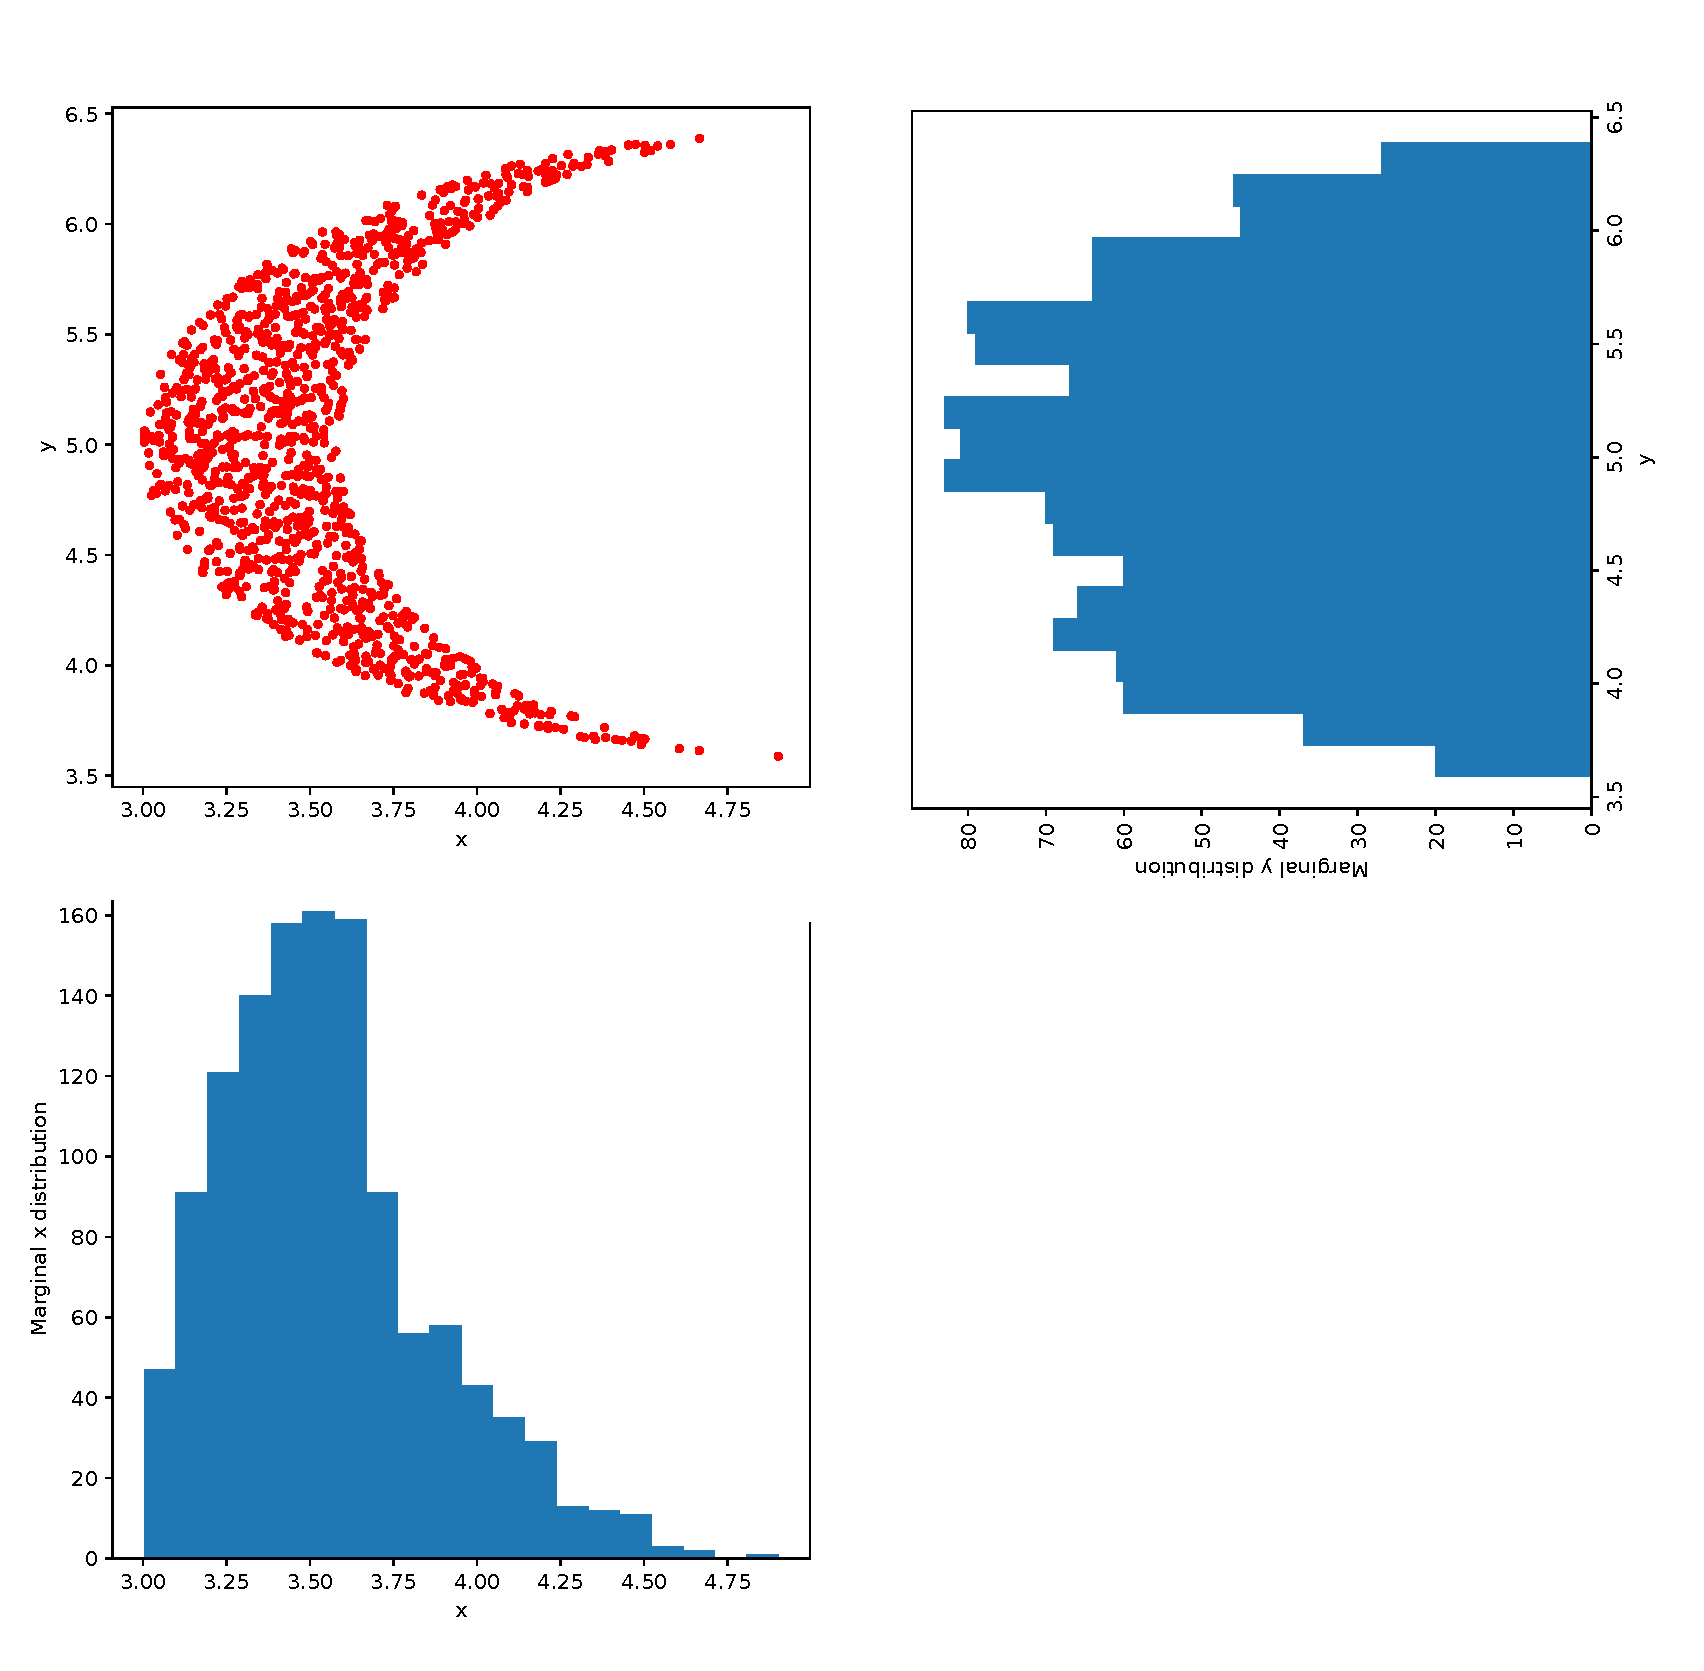
\includegraphics[width=0.7\textwidth]{jointmarge.pdf}
\end{center}
\caption{Joint probability distribution function in two variables $x$ and $y$. The marginal distributions are shown as a histogram in the margins of the joint distribution.}
\label{fig-jointmarge}
\end{figure}

It is important to realise that conditional and marginal probabilities in general convey substantially less information than the joint probability. Figure
\ref{fig-jointmarge} shows a joint distribution with a clear structure, but the marginal distributions broadly convey the extent of the data but not much more.
It is certainly not possible to infer the structure of the joint distribution from the marginal ones.

\begin{figure}[!h]
\begin{center}
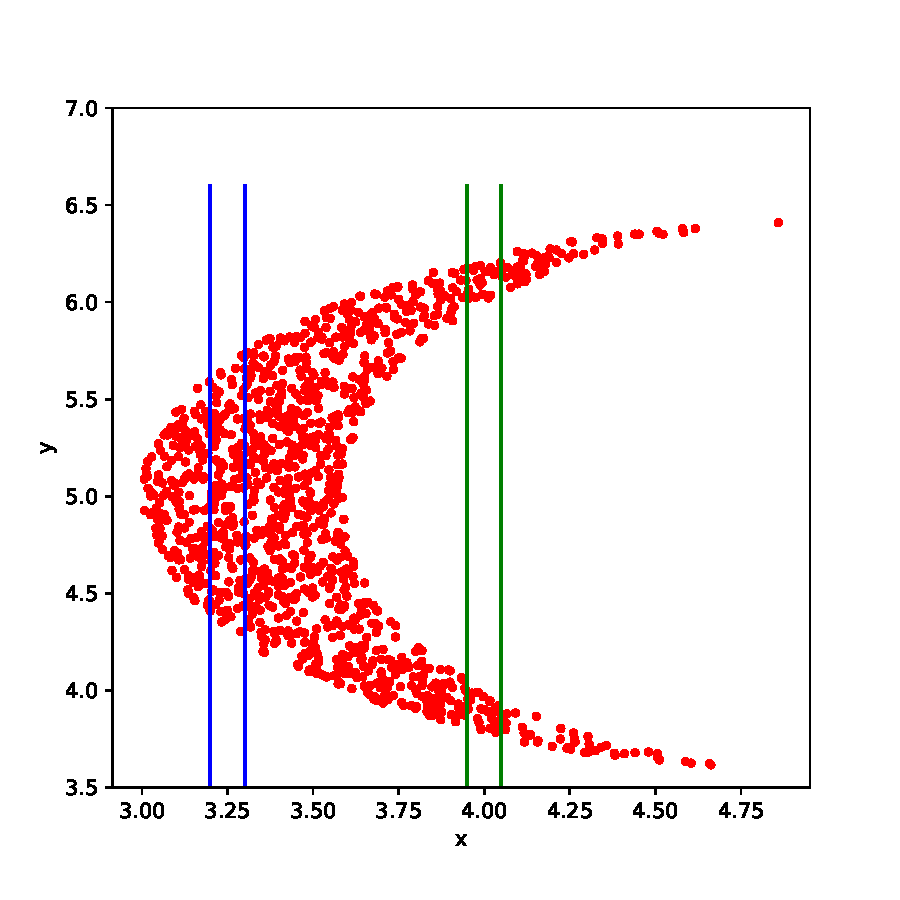
\includegraphics[width=0.4\textwidth]{jointcond.pdf}
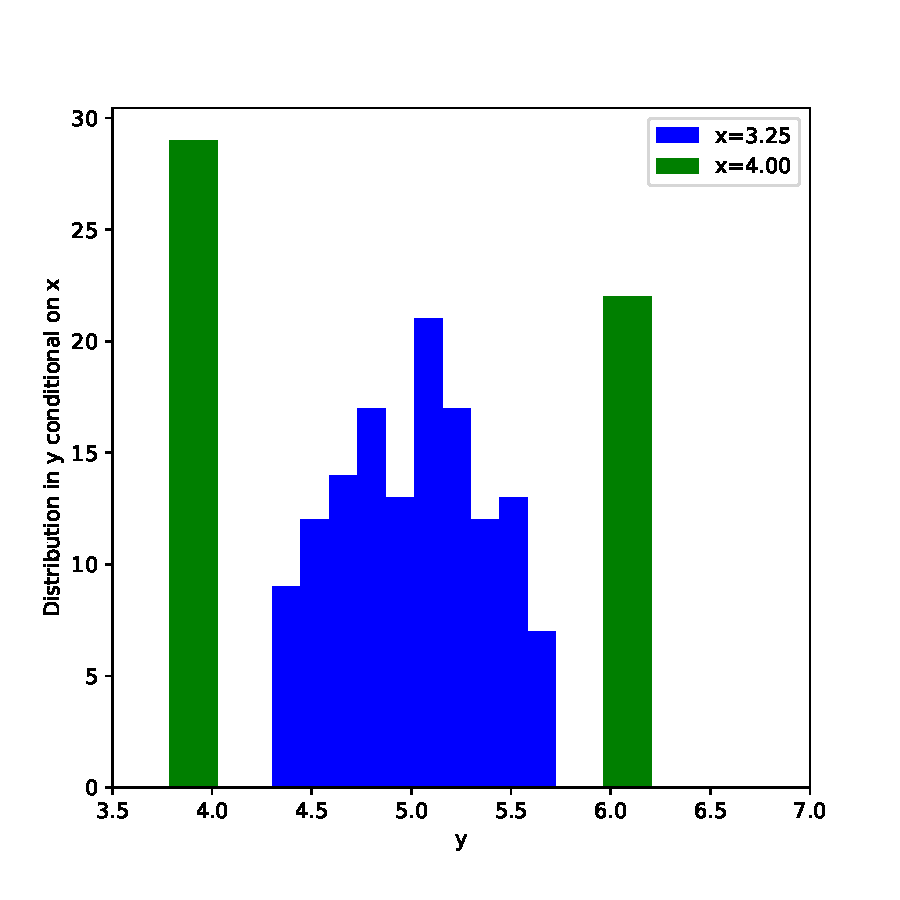
\includegraphics[width=0.4\textwidth]{ycond.pdf}
\end{center}
\caption{The same joint probability distribution conditioned on two different values of $x$. Each value of $x$ results in a one dimensional conditional distribution which can be unimodal or bimodal.}
\label{fig-jointcond}
\end{figure}

Conditioning the joint probability on one or more variables is similarly reductive.  Figure \ref{fig-jointcond} shows the same joint probability distribution, alongside with two one dimensional distributions which are obtained by conditioning the joint distribution on two different values
of $x$. The shape and properties of these distributions are clearly strongly dependent on which value of $x$ one chooses to condition on. It is also clear
that is impossible to reconstruct the original distribution. For that one would need the conditional distributions for all values of $x$.
  

\subsection{The Sum Rule and Product Rule}

The concepts introduced in the previous section are key to statistics and therefore machine learning. They amount to two rules:
The \emph{sum rule}:

\begin{equation}
P(X) = \sum_Y p(X,Y)
\label{eq-sum}
\end{equation}

The \emph{product rule}

\begin{equation}
P(X, Y) = p(Y \mid X)P(X)
\label{eq-product}
\end{equation}


\subsection{Bayes' Rule}
\label{sec-bayes}

Bayes' rule (sometimes called Bayes' law) relates conditional probabilities. Consider the product rule and observe that it may be written in two ways:
\begin{equation}
  P(X, Y) = P(Y  \mid X) P(X),
\end{equation}

or:

\begin{equation}
P(X, Y) = P(X \mid Y)P(Y)
\end{equation}

Inspecting Tab. \ref{tab-joint} makes plausible that these decompositions are equally valid.
It follows that:

\begin{equation}
P(X \mid Y) = \frac{P( Y \mid X)}{P(Y)}P(X)
\label{eq-bayes}
\end{equation}

or using the sum rule:

\begin{equation}
P(X \mid Y) = \frac{P (Y \mid X)}{\sum_X P(Y \mid X) P(X)} P(X)
\label{eq-bayesnormed}
\end{equation}

Both Eqs. \ref{eq-bayes} and \ref{eq-bayesnormed} are called Bayes' Rule, Bayes' Law (but not Baye's Rule).

On the one hand they reflect relatively trivial relationships between conditional probabilities. On the other hand they offer a tool that has had profound
impact on the development of statistics in the late 20th and 21st century. In particular, a consistent and systematic use of this rule avoids pitfalls in the analysis
of data. There are indications that we handle conditional probability well in everyday reasoning  if we use them to express \emph{causal} relationships,
but seriously mishandle them
if conditional probabilities do not express a causal relationship \cite{pearl2016,pearl2018}. Now please consider \emph{Unit1\_Activity\_Bayes} to see a real world example of the
relevance of Bayes' rule.

In the next section, we will provide a very simple example of Bayesian analysis of
a stochastic process.

\section{Bayesian Inference: an Unfair Coin}
\subsection{Introduction}

Imagine that we are predicting a series of coin tosses. Again, we model this with a Bernoulli process. A stochastic variable governed by a Bernoulli process has two possible outcomes: $\{ 0, 1 \}$ (we may associate 0 with 'head' and 1 with 'tails'). 
If $\mu = 0.5$ the coin is fair and if we throw $N=100$ times we may get a sequence of heads and tails. The individual elements of the throw may be unpredictable, but we expect approximately 50 heads and 50 tails.
If we were to see 25 heads and 75 tails we would have a hard time believing $\mu = 0.5$ and might guess it is closer to $\mu = 0.25$, which is the MLE.



\subsection{Bayesian Approach}
\label{sec-bayesexample}
The Bayesian approach requires us to make assumptions about the prior values of $\mu$. In the Bayesian view, probability corresponds to a subjective degree of believe.
In principle a coin can be weighted, and $\mu$ can take on any value. To simplify the situation, we assume that $\mu$ is discretised and can take on any of five values.

Since we know that $\mu$ can only assume five values, we must define a probability distribution over these values, the \emph{prior} distribution.
We could, for example,
assume that our opponent is most likely to be fair, but allow for some probability that the coin is unfair
in their advantage:


\begin{table}[!ht]
  \begin{center}
  \begin{tabular}{||c|c||}  \hline
    $\mu$ & $P_{prior}(\mu)$  \\ \hline  
    0.    &  0.05   \nonumber \\ 
    0.25  &  0.05   \nonumber \\
    0.50  &  0.7    \nonumber \\
    0.75  &  0.15   \nonumber \\
    1.0   &  0.05 \\ \hline
  \end{tabular}
  \end{center}
  \caption{The prior probabilities of a coin with 5 possible weighting values. It is most likely to be fair, but has small probabilities of being loaded.}
\end{table}


Our objective is to reassess these probabilities in light of a sequence of coin tosses that we have observed.
Bayes' rule gives us:

\begin{equation}
P(\mu = \mu_i \mid D ) = \frac{P(D \mid \mu_i)}{P(D)} P_{prior}(\mu = \mu_i)
\label{eq-posteriormu}
\end{equation}

Here $P(D \mid \mu_i)$ is simply the likelihood of the data as defined above:

$$
P(D \mid \mu_i) = \mu^{N_1}(1 - \mu_i)^{N - N_1},
$$

given $\mu$ it gives the probability of the observation of a particular sequence, which can be summarised in the only two numbers that are relevant: the number of 0 outcomes, $N_
0$, and the number of 1 outcomes $N_1$, from which we can compute $N= N_0 + N_1$.
Given a sequence of observations, we have the numbers to compute the posterior probabilities $P(\mu \mid D)$.


Now assume that we have observed 67 'tails' out of a 100 throws. This gives us all the numbers we need: $N_0 = 23, N_1 = 67, N= 100$
\begin{figure}[!ht]
\begin{center}
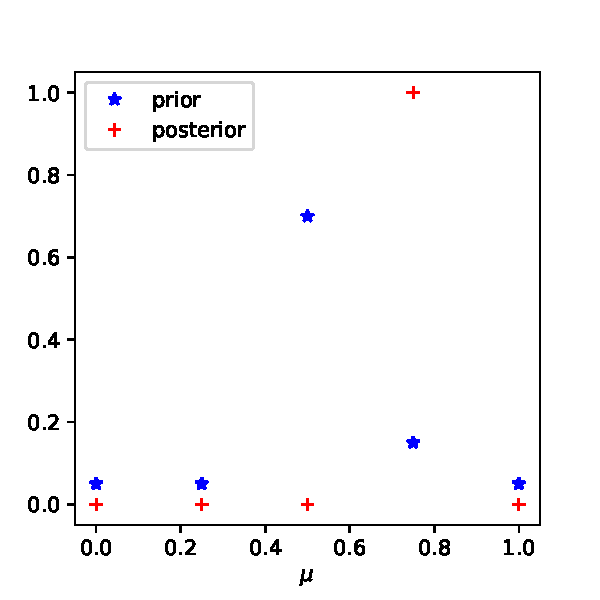
\includegraphics[width=0.7\textwidth]{falsecoin.pdf}
\end{center}
\label{fig-falsecoin}
\caption{The prior and posterior over a discrete set of $\mu$ values. The prior distribution was by our own choosing, reflecting the fact that we believed that the coin is fair, but allowing for uncertainty. The posterior distribution results from a consequent application of Bayes rule. It has shifted markedly to the right and now peaks nearly at the true value. The peak is relatively narrow, reflecting that we are now relatively confident.}
\end{figure}

Figure \ref{fig-falsecoin} shows both the prior and posterior probability. In the generation of the data sequence, we actually used $\mu = 0.75$, i.e. the outcome
of 75 tails would have been the most likely outcome. The posterior distribution peaks at closely this value and reflects that our estimate of $\mu$ has improved considerably.
The peak is also narrower, reflecting that we are more confident in our outcome.

The calculation has been performed in a Jupyter notebook called \emph{Unfair coins - Maximum Likelihood and Bayes}. You can experiment with different values of prior, number of throws and $\mu$ and observe the effect of these changes by running the notebook.


\subsection{The Complication of Normalisation}

Please note the following: it is relatively straightforward to calculate a given posterior probability for a single $\mu$-value \emph{up to a normalisation factor}:
$$
P_{posterior}(\mu = 0.5) \sim P( D \mid \mu)P_{prior}(\mu = 0.5)
$$

This is a lightweight calculation, given the simple form of the likelihood and that we know the prior. It is not apparent from this simple example that computationally the
biggest problem is the normalisation: we have to calculate $P(D)$ in Eq. \ref{eq-posteriormu}, and we can only do that by calculating $P(D \mid \mu_i)$ \emph{for all}
$\mu_i$. Alternatively, we can forego normalisation at first, ignoring the normalisation factor $P( D )$, but then we have to normalise the resulting outcomes. Either way,
we have to go through the process of calculating \emph{all} posterior outcomes, even if we're not interested in some of them! From this simple table example it will not
be clear why this is a problem. We will address it again when we have discussed conditional probability distributions, but this problem is a major obstacle
in the general application of Bayesian statistics!.





\subsection{Continuous Prior distributions}


In the example above, to illustrate the application of Bayes' rule to a table of conditional probabilities, we restricted the value of the $\mu$ variable to a number of discrete values. This demonstrates how simple the application of Bayes' rule really is, but a purist might complain that the maximum likelihood can take on any value, whereas the prior and posterior distribution are only defined on a small number of values, and therefore
we are not comparing like with like.

The continuous version is not fundamentally different, although it requires continuous prior and posterior
distributions over the interval $[0,1]$, thereby covering all values take $\mu$ could take potentially.
For continuous variables Bayes' rule is as follows:
$$
p(\mu \mid \mathcal{D} ) = \frac{p(\mathcal{D} \mid \mu)} {p(\mathcal{D})},
$$
where
$$
p(\mathcal{D}) = \int^1_0 p(\mathcal{D} \mid \mu )p(\mu) d \mu
$$

The main difference is that we now have to pick a continuous prior distribution. We could pick many, bearing in mind that it is supposed to express a prior belief about the value of the coin. If we firmly believe that $\mu = 0.5$ we should pick a prior that is sharply peaked around that value. If we are not firm in our belief, we could take a broader peak. If we believe the coin if false, we can take a value closer to 0 or 1.

As a functional form for the prior we use Beta function:
$$
\mbox{Beta}(\mu \mid a, b) = \frac{\Gamma(a+b)}{\Gamma(a)\Gamma(b)} \mu^{a-1} (1-\mu)^{b-1}
$$

The Gamma functions are a normalisation factor, which we will not discuss in detail here, but can easily be calculated using numpy. For positive integer values of $n$,
$\Gamma(n) = (n-1)!$.


The functional dependence is reminiscent of the likelihood. Remember that
for $N$ observations of which $N_1$ were '1' the likelihood is given by:
$$
p(\mathcal{D} \mid \mu)  = \mu^{N_1}(1 - \mu)^{N - N_1}
$$

Note the following:
\begin{enumerate}
\item The likelihood and the prior have a very similar form. This is deliberate: the computation of the posterior is very simple.
\item By picking variables $a$ and $b$ appropriately, we have great freedom in picking the shape of the prior. Helpful in this regard are the following relations:
\end{enumerate}
  
\begin{align}
\mathbb{E}(\mu) &= \frac{a}{a+b} \\
\mbox{var}(\mu) &= \frac{ab}{(a+b)^2(a+b+1)}
\end{align}

For example, the formula for the expectation shows that if you want your distribution to peak at $\mu =0.5$, you have to pick $a = b$.

We show the great variety of shapes that can be picked by selecting $a$ and $b$ appropriately:
\begin{figure}
\begin{center}
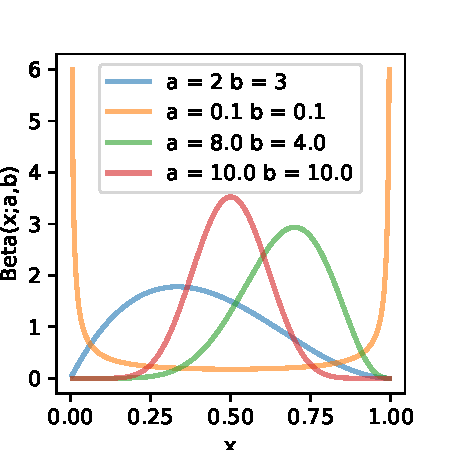
\includegraphics[width=0.7\textwidth]{beta.pdf}
\end{center}
\caption{The Beta distribution for several values of $a$ and $b$.}
\end{figure}


Applying Bayes' Theorem is remarkably straightforward:

Multiplying likelihood and prior, we obtain the posterior:
$$
p(\mu | \mid \mathcal{D} ) \sim \mu^{N_1 + a -1} ( 1 - \mu)^{N-N_1 + b - 1}
$$

Note:
\begin{enumerate}
\item The posterior is again a Beta function. The calculations shown here are greatly facilitated by a prior that plays nicely with the likelihood.
\item  The normalisation factor that isn't shown here can easily be calculated:
$$
\frac{\Gamma(N +a + b )}{\Gamma(N_1 + a ) \Gamma(N - N_1 + b )}
$$

\item  Using the formula for the expectation we can calculate that:
$$
\mathbb E[{\mu}]_{posterior} = \frac{N_1 + a}{a + b + N}
$$

\item In the limit of an infinite number of observations this is equal to $\frac{N_1}{N}$. In this limit the posterior will peak sharply around the maximum likelihood estimate.

\item For a finite amount of data, the expectation value of the posterior represents a compromise between the
(expectation of) the prior distribution and the maximum likelihood estimate.

\item  Since the parameters $a$ and $b$ essentially reflect the counts of the number of outcomes for $x=1$, $N_1$ and the total number of observations, $N$, the choice of prior can here be seen to be equivalent to artificially picking a number of prior observations by the modeller.

\item In Unit 2 we will  see that whilst the prior will generally be chosen such that prior times likelihood will result in the posterior having the same functional form as the prior, the prior usually does not have the same functional form as the likelihood.
\end{enumerate}

\begin{figure}
  \begin{center}
    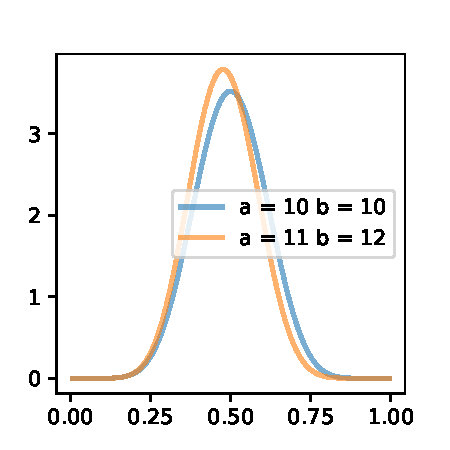
\includegraphics[width=0.7\textwidth]{posteriormu1.pdf} \\
    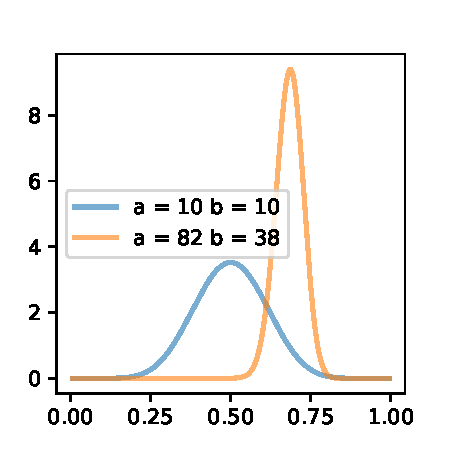
\includegraphics[width=0.7\textwidth]{posteriormu2.pdf} \\
  \end{center}
  \caption{Prior and posterior distributions after three observations of a heavily loaded coin $\mu = 0.75$, starting from a relatively broad prior centred around $\mu = 0.5$. Top: $N= 3$ observations, bottom $N=100$ observations.}
  \label{fig-postmu}
\end{figure}

We finish  with  a number of examples:
We use a highly loaded coin $\mu = 0.75$ $N=3$; prior $a=10, b= 10$, which corresponds to a prior that peaks around $\mu = 0.5$, i.e. initially we believed that our coin was
fair. The result is shown in Fig. \ref{fig-postmu} (top). We start with a fairly broad prior, centred around $\mu = 0.5$ reflecting a prior believe that the coin is balanced.
After three observations, we see that this prior has shifted slightly towards higher values, but has not changed substantially. We simply have not made a sufficient number
of observations. After $100$ observations(bottom), the picture has changed markedly: the posterior distribution peaks close to its true mean and is sharp, reflecting
a relatively high confidence in this value.

\subsection{Discussion}
It is important to compare the Bayesian analysis to maximum likelihood estimation. Consider that we have a true, but unknown value of $\mu = 0.5$ and that we are allowed to
observe the result of three throws only. This could easily be three tails, forcing us to conclude, on the basis of MLE that $\mu =1$. If we were to predict future
events, we would have to conclude that they only can be tails. No human observer would be confident in this: they would realise that three observations is not enough to base
such a stark conclusion on.

The Bayesian framework allows the inclusion of this prior uncertainty in a way that MLE does not. One could do sequence prediction on the basis of three observations
using the posterior distribution for $N=3$ in Fig. \ref{fig-postmu} top, and most human observers would agree this is a far more reasonable procedure. Even after 100 observations
there will be residual \emph{model uncertainty}. In a consequent application of the Bayesian framework this is an extra source of randomness in the parameters that determine
a process that is already stochastic. MLE on the hand produces a point value for these estimates.

A common procedure to try an estimate the uncertainty in MLE is \emph{cross validation}. In $k$-fold cross validation, the dataset is broken into $k$ partitions. Usually $k-1$
of those are involved in training the model and 1 of them is used to evaluate the model, a process that can be repeated $k$ times.

Bishop points out that the observation of three tails leads to \emph{overfitting} the MLE \cite{bishop2006}, and a three-fold cross validation would make no difference at all here.

Finally, the issue of normalisation has been treated casually here. The hard work has been done by introducing the Gamma function, but you are recommended to try  Exercise
2.5 in \cite{bishop2006} to appreciate that getting the normalisation right is possible because of the nice analytic properties of the Beta function and that without
such properties, or on an interval that is not $[0,1]$ we would have to resort to numerical integration. In a one dimensional distribution this is not a problem, but in
multivariate distributions this can become too expansive for practical purposes very rapidly.



  
  


  
